\subsection{Speeded-Up Robust Features (SURF)}
SURF is a method for both detecting and describing interest points in an image.
It outperforms earlier detection and description algorithms concerning repeatability, distinctivenss and robustness according to the work of \cite{SURF}.
The detection of interest points are calculated using the determinant of the Hessian matrix.
This matrix is produced by convolution of smoothing gaussian second derivatives with the image.
Here the points with local maximum of the determinant are declared as interest points, they represent {\it blob-like} features.

SURF's descriptor use two steps to extraxt robust features from an interest point.
First an orientation of the feature is calculated.
This will contribute to rotational invariance of the descriptor.
This orientation is used to form a square with the interest point in the center and from this square 64 features are calculated. using Haar Wavelets.
They are calculated using Haar Wavelets.
The Haar Wavelets are extracted by first calculating the sum of the intensity in two or more areas in an image.
Then a linear combinations of these intensities are calculated.
Using integral images these features can be calculated with just a few computations.
The interested reader if refered to \cite{SURF} and \cite{Viola2004}.

\subsection{Random Sample Consensus (RANSAC)}
As described in the work of \cite{RANSAC}, RANSAC is a robust method which can be applied in different applications with outliers in the data.
For example it is used to adapt models to find lines in point measurement such as fig. \ref{fig:theory:stitching:ransac}.
The method uses a random component which results in non deterministic output.
This stochasticity also connects the output to a probability and the goal is to create a high probabiliy of getting the {\it correct} output without any influence from the outliers.
To reach this goal there are multiple parameters to fine-tune.
For example, it is an iterative method and the number of iterations should be determined.
Each iteration randomly choose the minimun number of data points needed for calculating an output.
Then a value of how good these points represents the {\it correct} output is used to determine if these points are the best ones.
As mentioned this is repeated for a sufficient number of iterations.
Then the iteration that resulted in the best fit is set as the output from the method.

\begin{figure}[H]
  \centering
  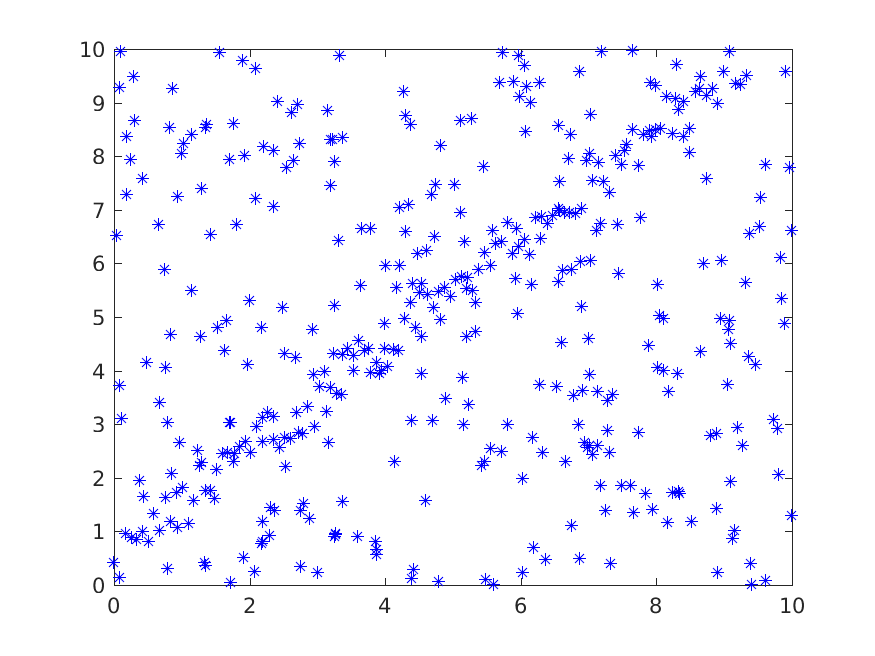
\includegraphics[width = .8\columnwidth]{../results/ransac.png}
  \caption{Example of problem to find the line in these data points which can be solved using RANSAC.}
  \label{fig:theory:stitching:ransac}
\end{figure}
